\documentclass{ximera}

\input{../../preamble.tex}

\author{Bobby Ramsey}

\begin{document}
\begin{exercise}

	Suppose $\theta$ is an acute angle fitting into the right triangle with sides as given in the following picture.\\
	\begin{center}
	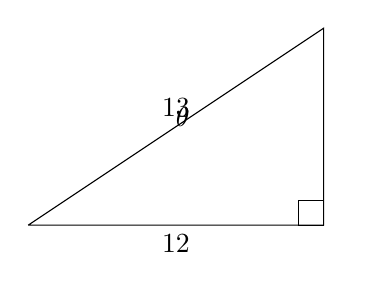
\begin{tikzpicture}[scale=1.25]
		\coordinate (C) at (-1.5cm,-1.cm);
		\coordinate (A) at (1.5cm,-1.0cm);
		\coordinate (B) at (1.5cm,1.0cm);
		\draw (C) -- node[above] {$13$} (B) -- node[right] {$$} (A) -- node[below] {$12$} (C);
		\draw (1.25cm,-1.0cm) rectangle (1.5cm,-0.75cm);
		\tkzMarkAngle[size=1cm,color=cyan,label=$\theta$](A,C,B)
		%\tkzMarkAngle[size=1cm,color=cyan,mark=|](C,B,A)
	\end{tikzpicture}
	\end{center}
	The length of the side opposite to $\theta$ is $\answer{5}$. 
	\begin{hint}
		Pythagorean Theorem
	\end{hint}
	\begin{exercise}
		Find the following trigonometric values.
		\begin{align*}
			\sin(\theta) &= \answer{5/13}\\
			\\
			\cos(\theta) &= \answer{12/13}\\
			\\
			\tan(\theta) &= \answer{5/12}\\
			\\
			\csc(\theta) &= \answer{13/5}\\
			\\
			\sec(\theta) &= \answer{5/13}\\
			\\
			\cot(\theta) &= \answer{12/5}\\
		\end{align*}
		\begin{hint}
			SOH-CAH-TOA
		\end{hint}
		\begin{exercise}
			The angle $\pi - \theta$ is in which quadrant?  What is its reference angle? 
			\begin{align*} 
				\text{ Quadrant } &=  \answer{2} \\ \\
				\text{ Reference Angle } &= \answer{\theta} \\
			\end{align*}
			
			\begin{exercise}
				\begin{align*}
					\sin(\pi-\theta) &= \answer{5/13}\\
					\\
					\cos(\pi-\theta) &= \answer{-12/13}\\
					\\
					\tan(\pi-\theta) &= \answer{-5/12}\\
				\end{align*}
			\end{exercise}
		\end{exercise}
	\end{exercise}
\end{exercise}
\end{document}